%% This is emulateapj reformatting of the AASTEX sample document
%%
\documentclass{article}


\newcommand{\vdag}{(v)^\dagger}
\newcommand{\myemail}{james.casey-clyde@sjsu.edu}

\usepackage{amsmath,amsfonts}
\usepackage[colorlinks]{hyperref}
\usepackage[numbers]{natbib}
\usepackage{graphicx}
\usepackage{caption}
\usepackage{subcaption}
\graphicspath{{../}}


%% You can insert a short comment on the title page using the command below.

%% If you wish, you may supply running head information, although
%% this information may be modified by the editorial offices.
%% The left head contains a list of authors,
%% usually a maximum of three (otherwise use et al.).  The right
%% head is a modified title of up to roughly 44 characters.
%% Running heads will not print in the manuscript style.

%% This is the end of the preamble.  Indicate the beginning of the
%% paper itself with \begin{document}.

\begin{document}

%% LaTeX will automatically break titles if they run longer than
%% one line. However, you may use \\ to force a line break if
%% you desire.

\title{Machine Learning in Gravitational Wave Analysis}
\author{J. Andrew Casey-Clyde}
\maketitle


%% Notice that each of these authors has alternate affiliations, which
%% are identified by the \altaffilmark after each name.  Specify alternate
%% affiliation information with \altaffiltext, with one command per each
%% affiliation.


%% Mark off your abstract in the ``abstract'' environment. In the manuscript
%% style, abstract will output a Received/Accepted line after the
%% title and affiliation information. No date will appear since the author
%% does not have this information. The dates will be filled in by the
%% editorial office after submission.

\begin{abstract}
Gravitational wave detectors such as LIGO and Virgo offer new insights into our universe, yet also present challenges for analysis, primarily due to the sensitivity of the detectors to terrestrial sources of movement, as well as to the volume of data generated by these detectors. However, given the natures of these challenges, they are well suited to machine learning solutions. In this paper, I present techinques for the identification of transient events in LIGO timeseries data on all channels, as well as techniques for classifying these events as either terrestrial or non-terrestrial in origin. 
\end{abstract}
%\twocolumn
\section{Introduction}
The search for gravitaional waves was a long one. Sparked in 1916 by Albert Einstein's theory of General Relativity, it wasn't until 100 years later, in 2016, that the first two gravitaitonal wave events were confirmed using data from Advanced LIGO's Hanford (H1) and Livingston (L1) detectors\citep{TheLIGOScientificCollaboration2016} \citep{Abbott2016}. LIGO's instruments yield large quantities of data, which can be a double edged sword from an analysis perspective. The data is also subject to large amounts of terrestrial noise, which may be confused for transient gravitational wave events. This makes the data difficult for manual examination, so instead we turn to clustering and machine learning techniques, which offer powerful tools for extracting meaning from all this data.

In this paper, I apply the Kliene Welle algorithm\citep{Chatterji2004}\citep{Blackburn2007} to the first two weeks of LIGO's S6 data release, which uses clustering to find energy overdensities in gravitational wave timeseries and identify transient events. I then use a Multi-Layer Perceptron (MLP) neural network to classify these events, with LIGO hardware injections serving as simulations of various classes of gravitaitonal waves.

\section{Methods}
In order to classify transients in the LIGO data, they must first be found. To this end, I apply the Kleine Welle algorithm, which decomposes wavelets into the time-scale domain and searches for regions of energy overdensities in the signal\citep{Biswas2013}\cite{Blackburn2007}. These techniques may be applied to all detector channels to extract transients, and in fact will be necessary for differentiating between terrestrial and astrophysical transient sources.

\subsection{Data Cleaning}
The LIGO gravitational wave data is characterized by Gaussian noise, with non-Gaussian transient events. As such, before applying the Kleine Welle algorithm to search for overdensities, it is useful to first whiten the data by taking it's Fourier transform and dividing by the amplitude spectral density (ASD), which is the square root of the power spectral density, and then transforming back\citep{LIGOScientificCollaboration}. This helps to suppress signal due to noise, enhancing transient signals. An example of strain data pre and post whitening and bandpassing is shown in Figure \ref{fig:cleaning}, and it's ASD at all stages of the cleaning process in Figure \ref{fig:asd}.

\begin{figure}
\begin{subfigure}[t]{0.5\textwidth}
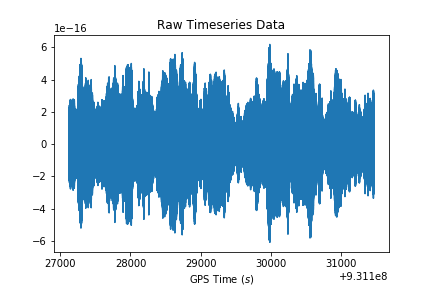
\includegraphics[width=\textwidth]{dirty.png}
\caption{Strain data before whitening}
\label{fig:dirty}
\end{subfigure}
\begin{subfigure}[t]{0.5\textwidth}
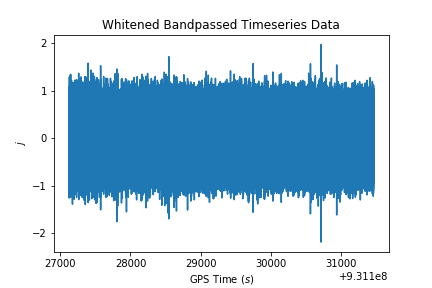
\includegraphics[width=\textwidth]{clean.png}
\caption{Strain data after whitening and applying a butterworth bandpass filter}
\label{fig:clean}
\end{subfigure}
\caption{Strain data for a section of LIGO S6 data. The cleaned data has been whitened by dividing it's fourier transform by it's ASD, and then had a butterworth bandpass applied from $80-300\mathrm{Hz}$}
\label{fig:cleaning}
\end{figure}

\begin{figure}
\begin{subfigure}[t]{0.5\textwidth}
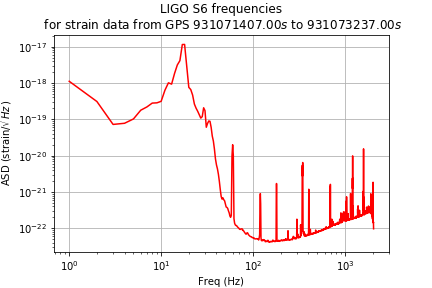
\includegraphics[width=\textwidth]{noise.png}
\caption{ASD before whitening}
\label{fig:prewhite}
\end{subfigure}
\begin{subfigure}[t]{0.5\textwidth}
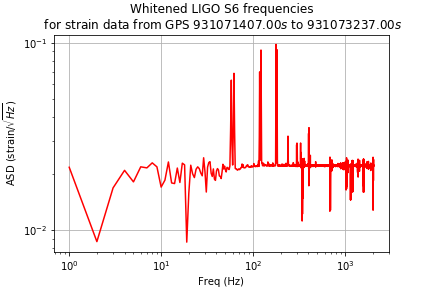
\includegraphics[width=\textwidth]{white.png}
\caption{ASD after whitening}
\label{fig:postwhite}
\end{subfigure}

\begin{subfigure}[t]{0.5\textwidth}
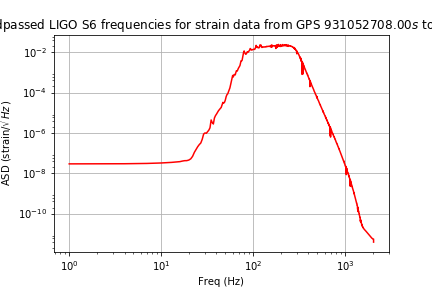
\includegraphics[width=\textwidth]{whitebp.png}
\caption{Whitened ASD with a butterworth filter applied at critical frequencies $80\mathrm{Hz}$ and $300\mathrm{Hz}$}
\label{fig:postwhitebp}
\end{subfigure}

\caption{ASD vs. frequency for a segment of LIGO S6 data, before and after whitening. Notice that in about the $80-300\mathrm{Hz}$ range, the noise is at a minumum, and relatively constant. This is the range we wish to search for transient events.}
\label{fig:asd}
\end{figure}

Additionally, a butterworth bandpass filter may be applied to the whitened data\citep{Blackburn2007}\citep{LIGOScientificCollaboration} in order to remove regions of large or fluctuating background noise, such as those regions outside $80-300\mathrm{Hz}$ in Figure \ref{fig:prewhite}.

\subsection{Event Identification}
Once the data has been whitened and bandpassed, it can be fed through the Kleine Welle algorithm. The algorithm works through the application of a dyadic wavelet decomposition, whose coefficients can be used to search for signal energy overdensities\citep{Biswas2013}\citep{Blackburn2007}. In general, the wavelet transform is defined by the equation\citep{Blackburn2007}\citep{Mallat1999}
\begin{equation}
W_{f}(u,s)=\int_{-\infty}^{+\infty}f(t)\frac{1}{\sqrt{s}}\psi^{*}\left(\frac{t-u}{s}\right)dt, \label{eq:wavtr}
\end{equation}
where $s$ is the scale. The calculation of this transformation can be made computationally inexpensive through the discretization of $s$ to a dyadic sequence, such that $s \in \{2^{j}\}_{j\in\mathbb{Z}}$\citep{Blackburn2007}\citep{Mallat1999}.

Applying this to the LIGO timeseries data at multiple scales (where we now switch to $j$, for convenience in the dyadic series) yields a series of detail coefficients $D_{j}$ for each scale, with elements $d_{ij}$, whose values scale with signal energy and approach a zero mean Gaussian\citep{Blackburn2007}. We can threshold on these elements to look for outliers by using the standard deviation of each decomposition level, $\sigma_{j}$, such that $d_{ij}/4\sigma_{j} > 4$. Elements which pass this threshold are then normalized to create a set of square normalized coefficients such that
\begin{equation}
E_{j} = D_{j}^{2}/\sigma_{j}^{2} = \{\epsilon_{ij}\},
\end{equation}
where the elements $\epsilon_{ij}$ correspond to the same elements $d_{ij}$. Taking only those $\epsilon_{ij}$ whose corresponding detail coefficients passed the earlier thresholding, we can cluster these over time, decomposition scale, and normalized energy. The mean shift clustering method is particularly well suited to this problem, as it does not require prior knowledge or the number of clusters present\citep{Ivezic2014}, which in principle we cannot know for a given segment. An example of this clustering is shown in Figure \ref{fig:cluster}. The elements of a given cluster $C$ can then be added to form the total normalized cluster energy\citep{Blackburn2007},
\begin{equation}
E_{c} = \sum_{(i,j)\in C}\epsilon_{ij}. \label{eq:Ec}
\end{equation}
The significance of a cluster is then defined as\citep{Blackburn2007}
\begin{equation}
S=-\ln\int_{E_{c}}^{+\infty}\chi_{N}^{2}(E)dE, \label{eq:significance}
\end{equation}
where the number of degrees of freedom $N$ is the number of elements in the cluster. With this, it simply becomes a matter or thresholding the significance of each cluster.

\begin{figure}
\begin{subfigure}[t]{\textwidth}
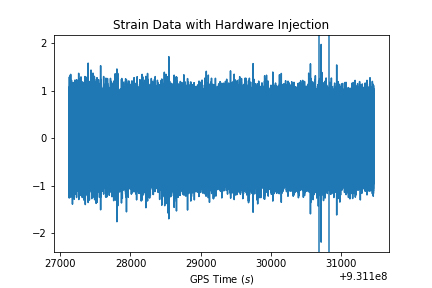
\includegraphics[width=\textwidth]{hw_strain.png}
\caption{Strain data with hardware injection}
\label{fig:hw_strain}
\end{subfigure}

\begin{subfigure}[t]{\textwidth}
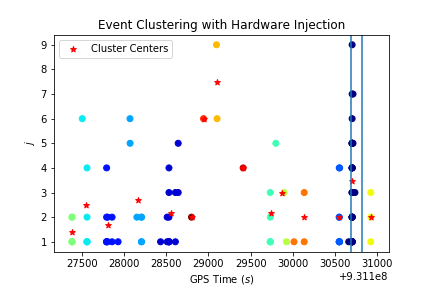
\includegraphics[width=\textwidth]{cluster.png}
\caption{Clustering in time and scale, including cluster centers. Each cluster represents a transient event.}
\label{fig:cluster}
\end{subfigure}
\caption{Clustering in time and scale for a section of strain data that includes a hardware injection. Blue bars in both images mark the start and end of the hardware injection period.}
\label{fig:event}
\end{figure}

\subsection{Event Classification}
Once transients have been identified in the strain data, they can be classified using a neural network; in this case, I choose to use a Multi-Layered Perceptron, one of the more popular neural networks. For training data, we can use hardware injected events for astrophysical event classification. Additionally, we also need non-astrophysical events to train on. These can be generated by looking for events in each detector that do not overlap with events from the other detector (i.e., events in H1 that do not overlap with events from L1). By applying the hardware injections and independent events as labels, we can then form a set of data for training and testing.

\section{Analysis}
Keeping in mind that each LIGO science run contains data collected using progressively more sensitive instruments, I choose to apply these techniques to the first two weeks of the S6 data release\citep{LIGOScientificCollaboration2015}, from the most recent data collection run before Advanced LIGO instruments came online, which offers the best sensitivity for publically available data. This data has been downsampled (by LIGO) from $16384\mathrm{Hz}$ to $4096\mathrm{Hz}$\citep{LIGOScientificCollaboration2015}. The data files must be cached locally, so local storage availability is a factor when determining how much data may be examined. The data files themselves contain strain data in the form of a timeseries, as well as meta data, including channels indicating when hardware injections of simulated gravitational wave data were active. These data files are loaded as a series of time segments using LIGO's readligo python module\citep{Kanner2017}, with each data segment being run through a Kleine Welle algorithm as described above.

Wavelet decomposition (eq. \ref{eq:wavtr}) is carried out using the open source PyWavelets package\citep{Wasilewski}. The detail coefficients, $D_{j}$, are then examined at each scale $j$, and statistically significant ($d_{ij} > 4\sigma_{j}$) points are found. These points are clustered in time, scale, and square normalized energy, $\epsilon_{ij}$, into event clusters using a Mean Shift algortihm. The significance of each cluster (as defined by equations \ref{eq:Ec} and \ref{eq:significance}) is then calculated, and events with a significance under $20$ are discarded. When a significant cluster ($S > 20$) is found, it is recorded in a data file, with start and end times, event length, the significance of the event, and the cluster center (in time, scale, and energy). Using this technique, I find 698 events from H1, and 809 events from L1.

In order to make use of a classification neural network, we first need labeled data to train it with. The S6 LIGO data includes injection time periods, i.e. when and for how long each type (Compact Binary Coalescence (CBC), Burst, and Stochastic) of hardware injection was active, which can be used to generate this labeled data. By comparing these activation periods to the start and end times of each detected event, we can identify which of our events correspond to hardware injections. Additionally, we can use the hardware injection data to count the number of injections, to gauge how well we can detect injections. In this portion of the season S6 data, there exist 7 CBC injections and 1 Burst injection in H1, and 3 CBC and 2 Burst injections in L1 (with no Stochastic injections in either detector). Comparatively, The Kleine Welle algorithm is able to pick out 20 CBC and 1 Burst cluster in H1, and 1 CBC and 2 Burst clusters in L1. While the Burst data is very consistently picked up by the clustering algorithm, the number of CBC injections found is very sensitive to the clustering bandwidth used. Further improvements to these methods should start here, potentially using a clustering method that is better able to handle arbitrary numbers of clusters of very different sizes. Additionally, we can confirm some events as being terrestrial in origin by comparing the data from each detector, H1 and L1, to each other and looking for events which do not overlap in time, $\pm100\mathrm{ms}$, following the same time window used by Biswas, et al\citep{Biswas2013}. In total, I find 3479 terrestrial events in this data.

All identified events can then be labeled and used for training and testing the neural network. For neural network model, I choose to use a Multi-Layer Perceptron (MLP), though in principle, any neural network which can be trained for classificaiton will work. To characterize the performance of the MLP, I apply cross validation to  the labeled data containing all of the injected events with $k=10$, getting a score of $0.99\pm0.03$, though it should be noted that this value tends to skew high, due to the large number of terrestrial events.

By applying the MLP to the H1 and L1 data seperately, these events may be validated against each other to find gravitational wave candidates. However, in applying this I find no non-terrestrial events. Considering the section of data used, this is more likely due to necessitating further refinements to the clustering process, and could also likely be helped with a larger section of data containging more injections.

\section{Conclusion}
Machine learning offers powerful tools for dealing with the vast quanitities of data that need to be searched for gravitational waves. As more detectors come online, and the sensitivity and time resolution of these detectors increase, techniques such as these will become invaluable in the search for gravitational waves. In particular, the Kleine Welle algorithm seems to do well in finding events, and is able to find all injected events, offering a method whose parameters may only need to be tuned to the data set. MLP Neural networks also offer promise in categorizing transient events, achieving a score of $0.99\pm0.03$. It should be noted, however, that the section of data explored did not contain a large number of injections. A more focused exploration of these techniques with data from more injections would be worth merit (this study was unfortunately limited by available hardware to a smaller section of the overall data).

\bibliography{library}
\bibliographystyle{unsrt}


\end{document}

%%
%% End of file `sample.tex'.
